\documentclass{beamer}
\usetheme{CMU}

\usepackage{pgf,pgfarrows,pgfnodes,pgfautomata,pgfheaps,pgfshade}
\usepackage{amsmath,amssymb}
\usepackage[utf8]{inputenc}
\usepackage{colortbl}
\usepackage[english]{babel}
\usepackage{booktabs}
\usepackage{slpython}
\usepackage{underscore}

\author{Luís Pedro Coelho}
\institute{Programming for Scientists}

\graphicspath{{figures/}{figures/generated/}{images/}}

\newcommand*{\code}[1]{\textsl{#1}}


\title{GUI Programming (II)}
\begin{document}
\frame{\maketitle}

\begin{frame}[fragile]
\frametitle{Where Were We?}
We saw that the basics elements of a GUI program were
\begin{itemize}
\item widgets
\item event loop
\item signals \& slots
\end{itemize}
\end{frame}

\begin{frame}[fragile]
\frametitle{Widgets}

\centering
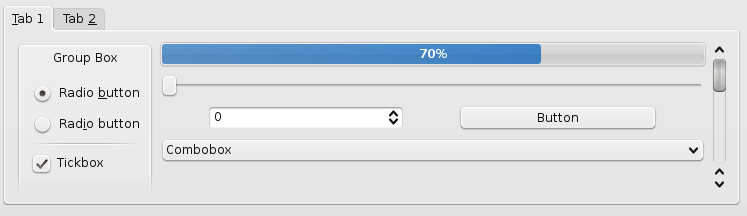
\includegraphics{widgets}

\end{frame}

\begin{frame}[fragile]
\frametitle{Widgets}

\centering
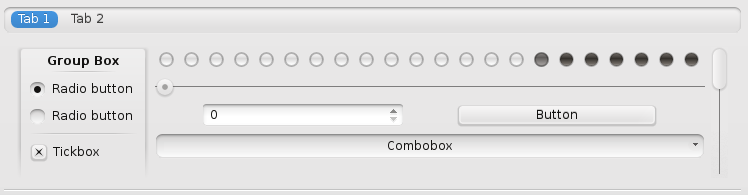
\includegraphics{widgets-bespin}

\end{frame}

\begin{frame}[fragile]
\frametitle{Widgets}

\centering
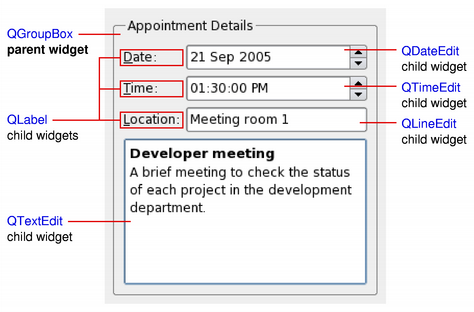
\includegraphics{parent-child-widgets}

\creditto{Qt Documentation}

\end{frame}

\begin{frame}[fragile]
\frametitle{Advanced Widgets}
\begin{itemize}
\item Webkit widget
\item Qwt: technical widgets for Qt
\item Matplotlib
\item \ldots
\end{itemize}
\end{frame}

\begin{frame}[fragile]

\bigskip
\bigskip
\bigskip
Let's build a more complex \textsc{gui}\ldots
\end{frame}

\begin{frame}[fragile]
\frametitle{What About the Quit Button?}
\begin{python}
app.connect(main.actionQuit,QtCore.SIGNAL('activated()'),app.quit)
\end{python}
\end{frame}

\begin{frame}[fragile]
\frametitle{What About Doing Something?}

For a lot of applications, we're done.

For scientific applications, not so much.
\end{frame}

\begin{frame}[fragile]
\frametitle{Doing Something Complicated}
\begin{itemize}
\item Do a bit here and there\\
    checking for user events.
\item Start another process
\item (Start another thread)
\end{itemize}
\end{frame}

\begin{frame}[fragile]
\frametitle{Starting Another Process}
\begin{python}
from PyQt4 import QtCore, QtGui
app = QtGui.QApplication(sys.argv)

button = QtGui.QPushButton('Press Me')
button.setWindowTitle('Hello')
button.show()


\end{python}

\end{frame}
\begin{frame}[fragile]
\frametitle{Starting Another Process (II)}
\begin{python}

proc = QtCore.QProcess()
def process_output():
    output = proc.readAllStandardOutput()
    print 'output from process >>', output, '<<'

def startit():
    proc.start('python',['sleeper.py','10'])

app.connect(proc,QtCore.SIGNAL('readReadyStandardOutput()'),process_output)
app.connect(button, QtCore.SIGNAL('clicked()'),startit)

sys.exit(app.exec_())
\end{python}
\end{frame}

\begin{frame}[fragile]
\frametitle{One Final Note: Distribution}
\begin{itemize}
\item Pyinstaller
\item py2exe
\end{itemize}
\end{frame}
\end{document}
